\section{Introduction}\label{Intro}
\begin{figure}[h]
    \centering
    \vspace{-0.2cm}
    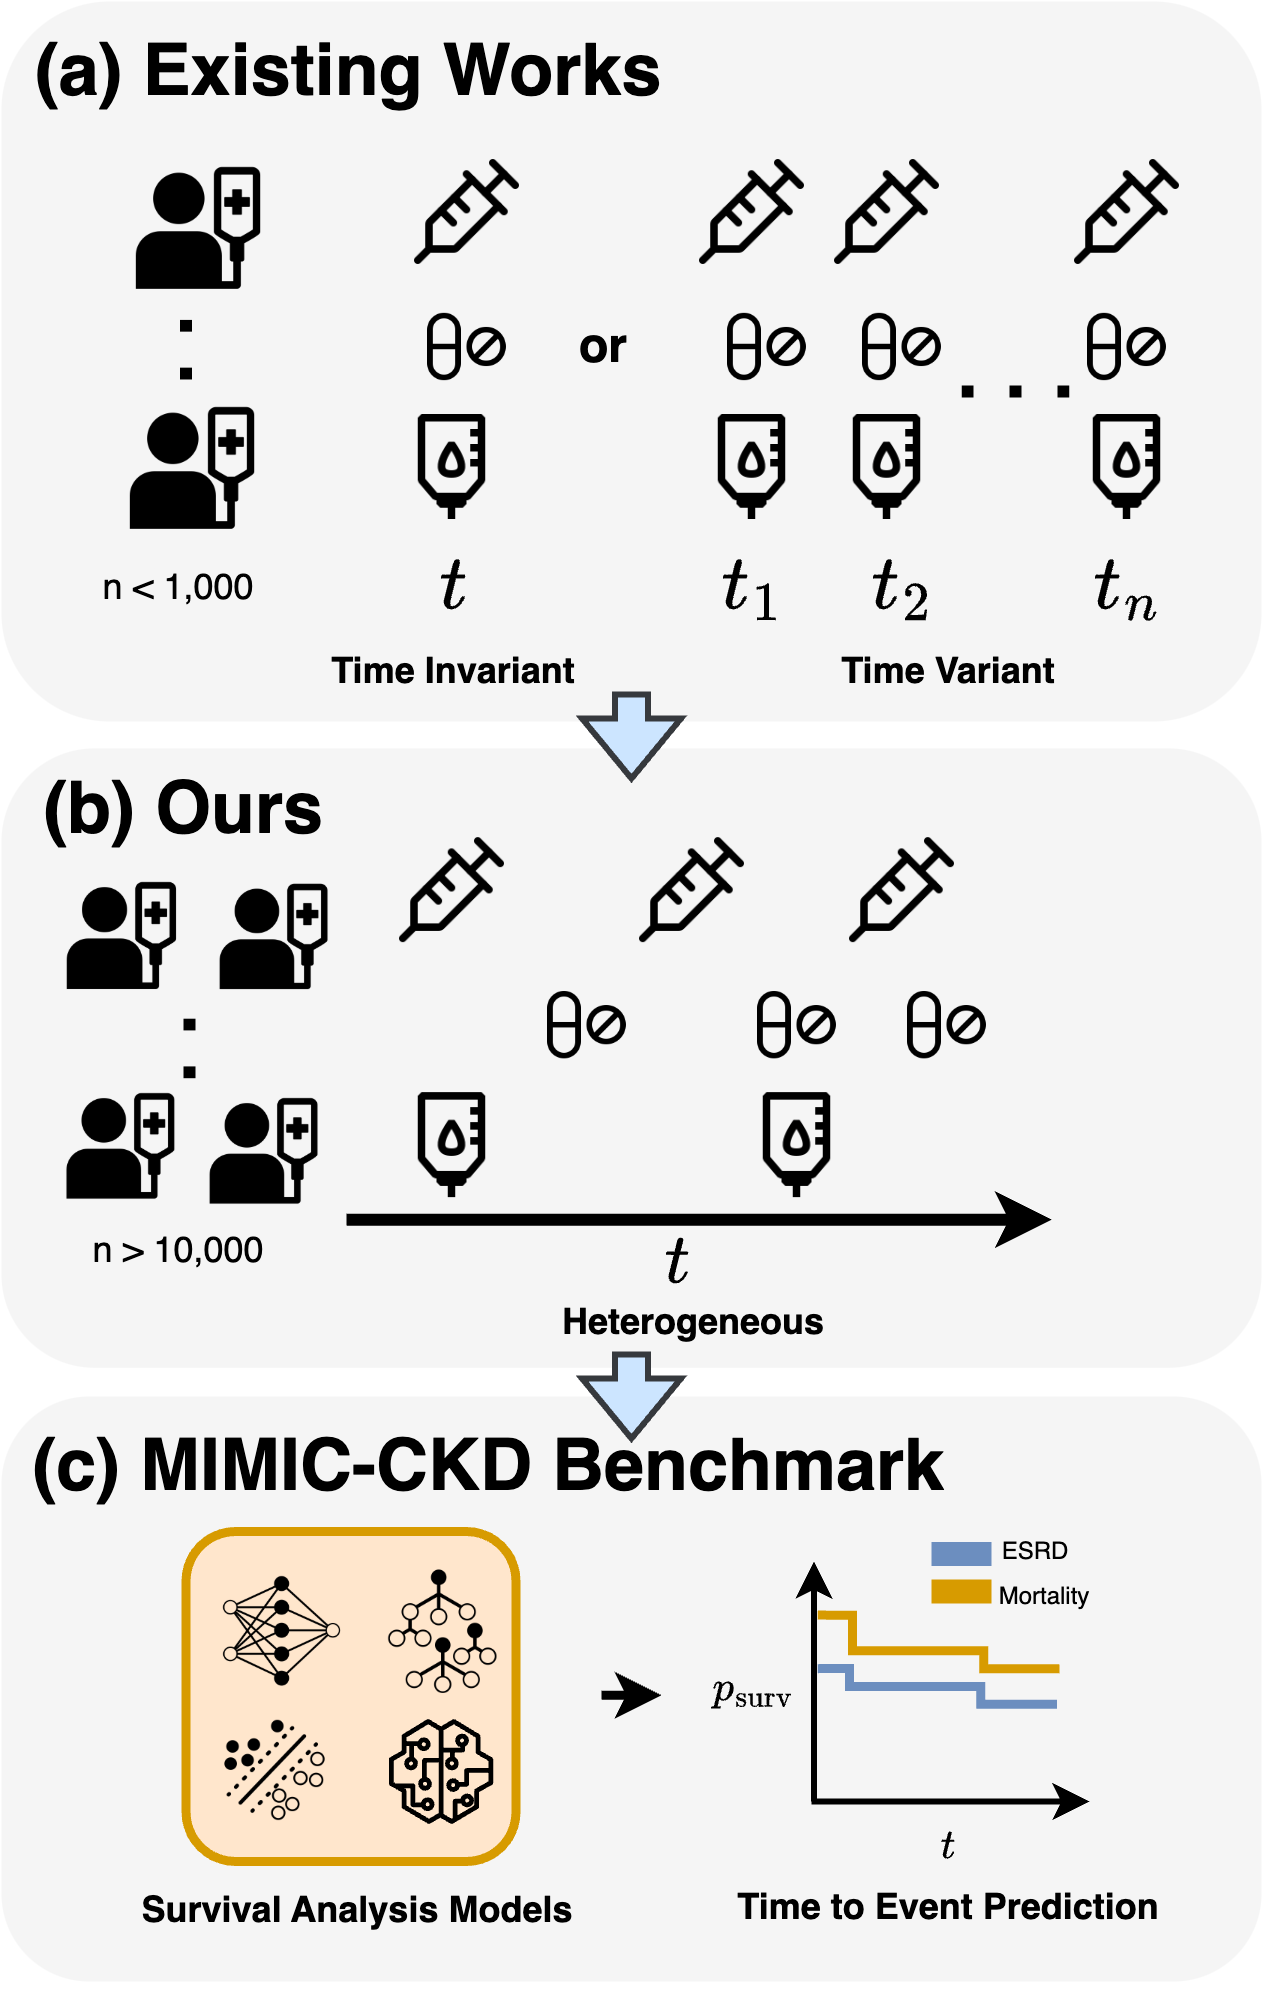
\includegraphics[width=0.45\textwidth]{figs/PatientProfile.drawio.png}
    \caption{Patient profiles are often heterogeneous and complex in clinical settings. They vary considerably in the number of available features and time points of data collection. Leveraging this information to predict CKD progression is nontrivial. (a) In existing works surrounding CKD-ESRD time to event prediction, we observe that many ignore this environment and either assume time invariance \citep{swain2023robust_classifier_imputation_CKD} or uniform monitoring of lab events \citep{chen2019ckd_diagnosis} across a small set of publicly available patient data. (b) Our benchmark explores the challenge of incorporating features that are not only missing across different patient profiles, but also across different time points among a much larger set of patients. (c) We explore the performance of various existing cited survival analysis models in our MIMIC-CKD benchmark.}
    \label{fig:CKD_benchmark}
    \vspace{-0.2cm}
\end{figure}
Chronic kidney disease (CKD) affects over 1 in 7 Americans \citep{CDC2023CKD} and is frequently associated with cardiovascular complications including stroke and heart disease \citep{said2014link_cardiovasc}. CKD can progress to end-stage renal disease (ESRD), which has a five-year survival rate below 50\%. While early intervention is critical for preventing ESRD \citep{levin2011early_detection}, predicting CKD progression remains challenging due to its ambiguous definition and often asymptomatic nature \citep{zhong2017perspective_CKD_biomarkers}.
To identify reliable biomarkers of disease progression, various predictive models have been trained for CKD. In mining electronic health records (EHR) to better understand associated features with CKD, \cite{chicco2021machine_CKD_analysis} find highly correlated biomarkers like age, eGFR, and creatinine, but more remarkably find that other temporally-relevant conditions like hypertension. smoking, and diabetes progression directly affect CKD. The significance of temporal features aligns with evidence that CKD risk increases with age \citep{hill2016global_Survey_CKD}. This temporal dimension is particularly relevant in clinical settings, where kidney function is monitored through recurring blood and urine tests, especially for diabetes-related complications \citep{chen2019ckd_diagnosis}. However, the varying importance of different features across studies highlights a critical gap between controlled research environments and real-world clinical scenarios, where patient data is often heterogeneous and incomplete across time points \citep{wu2024multimodal_missing_modalities} as depicted in Figure \ref{fig:CKD_benchmark}. 

 While many studies have performed CKD survival analysis, their datasets are either private \citep{fatin2023renal_saudi_analysis_example1_of_private_data}, have been conducted on a very small time-invariant scale (i.e less than 1,000 patients) \citep{swain2023robust_classifier_imputation_CKD}, or fail to consider a wider range of features available within EHR.

As such, it is crucial to build a benchmark that leverages a more comprehensive set of features and outcomes. We construct a new dataset analyzing CKD progression from MIMIC-IV \citep{johnson2023mimic_ehr}. 

To the best of our knowledge, our benchmark is the first to:

\begin{itemize}
    \item Include a large-scale cohort of over 10,000 patients across 50,000 clinical visits
    \item Capture realistic patient trajectories through temporally heterogeneous clinical features
\end{itemize}

We benchmark our dataset MIMIC-CKD across a wide variety of methods, including deep neural network survival models that can encode nonlinear relationships between the covariates and predicted outcomes such as DeepHit \citep{lee2018deephit}, Dynamic DeepHit \citep{lee2019dynamic_deephit}, RNN-Surv \citep{giunchiglia2018rnn_surv}, Hazard Transformer \citep{hazard_transformer}, as well as more traditional techniques such as Cox models \citep{cox1972regression}, gradient boosted machines \citep{chen2013gradient_GBSA}, and survival random forests \citep{pickett2021random_survival_forests}. We observe that deep models on average outperform their traditional counterparts and scalably incorporate more features, improving performance upwards of 20\%. 

% \begin{figure*}[h!]
%     \centering
%     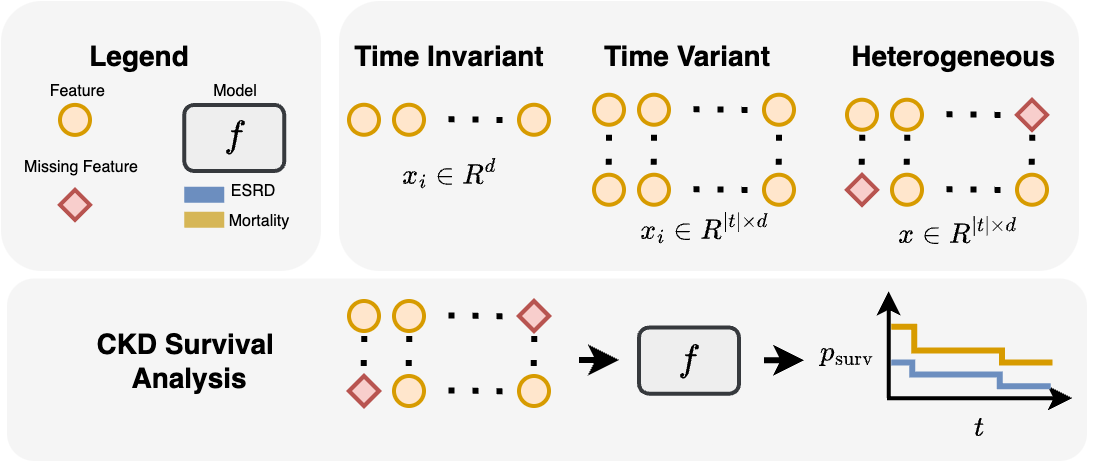
\includegraphics[width=1.0\textwidth]{figs/CKD_Benchmark_Horizontal.drawio.png}
%     \caption{Three scenarios commonly persist in survival analysis works. (1) Time Invariant: There exists no temporal component to co-variates where we effectively take a slice of time for each patient. (2) Time Varying: We take multiple time points and assume all features are visible. (3) Heterogeneous: where we observe both multiple time points and missing features depending on the time point or visit. We note that the large-scale clinical dataset MIMIC and real-world clinical pipelines typically mirror that of the heterogeneous setup \cite{wu2024multimodal_missing_modalities}.}
%     \label{fig:CKD_benchmark}
% \end{figure*}

% insert literature review

% Article on CKD Classificaiton, more related work
% https://pmc.ncbi.nlm.nih.gov/articles/PMC10201999/


% insert literature review of all models that are used here. 
% insert how our model is using those features and more, including the temporal components, and accounting for heterogeneity, which is common in hospital/clinical setings.